\documentclass[conference]{IEEEtran}
\usepackage{graphicx,times,amsmath,algorithm,caption, subcaption,nicefrac,bm}
\usepackage{multicol}
\usepackage[noend]{algpseudocode}
\usepackage{mathtools}
\usepackage{bbm}
\usepackage{amssymb}

\pdfminorversion=3

\newcommand{\defeq}{\vcentcolon=}
\newcommand{\eqdef}{=\vcentcolon}
\newcommand{\mathsc}[1]{{\normalfont\textsc{#1}}}
\newcommand{\argmax}{\operatornamewithlimits{argmax}}
\DeclareMathOperator*{\argmin}{arg\,min}
% correct bad hyphenation here
\hyphenation{op-tical net-works semi-conduc-tor}
% % \usepackage[table]{xcolor}

\DeclareMathOperator{\dis}{d}
\DeclarePairedDelimiter{\ceil}{\lceil}{\rceil}


\newcommand{\twopartdef}[4]
{
	\left\{
		\begin{array}{ll}
			#1 & \mbox{if } #2 \\
			#3 & \mbox{otherwise } 
		\end{array}
	\right.
}

\IEEEoverridecommandlockouts

\begin{document}

% Paper title: keep the \ \\ \LARGE\bf in it to leave enough margin.
\title{\ \\ \LARGE\bf Rolling Horizon methods for Games with Continuous States and Actions } 
% TODO - better title

\author{Samuel A. Roberts, Spyridon Samothrakis, Diego Perez, Simon M. Lucas}

% Uncomment out the following line for invited papers
%\specialpapernotice{(Invited Paper)}

% Make the title area
\maketitle


\begin{abstract}
It is often the case that games have continuous dynamics and allow for continuous actions, possibly with with some added noise. For larger games with complicated dynamics, having agents learn offline behaviours in such a setting is a daunting task. On the other hand, provided a forward model is available, one might try to spread the cost of search/learning in a rolling horizon fashion (e.g. as in Monte Carlo Tree Search). In this paper we compare T-HOLOP (Truncated Hierarchical Open Loop Planning), an open loop planning algorithm at least partially inspired by MCTS with a version evolutionary planning using CMA-ES (which we call EVO-P) in two planning benchmark problems (Cart Balancing and the Double Integrator) and Lunar Lander, a classic arcade game. He show that EVO-P outperforms T-HOLOP in almost all settings. We conclude that off-the-shelf evolutionary algorithms can be used successfully in a rolling horizon setting, and might offer considerable advantages over more formal methods. 

\end{abstract}

% No keywords



\section{Introduction} \label{Introduction}
One of the most common uses of function optimisation is for solving control problems. If an agent has access to a generative model of the world (i.e. a simulator) in which it is going to act, a control problem becomes a search/optimisation problem, usually referred to as ``simulation based planning''. Recently, a family of algorithms, mostly known as Monte Carlo Tree Search (MCTS)~\cite{browne2012survey}, has been applied to planning problems of discrete states and actions with considerable success. The focus of these algorithms is to attack extremely large state spaces of perfect information games, where one can sample rewards from the state space easily (e.g. Computer Go~\cite{gelly2006modification}). With access to a generative model (from which one can easily sample) and perfect sensor information, the following procedure works well: the agent receives sensor information, formulates a plan of action, performs the first action of that plan, receives a new state, re-formulates a plan, acts again (using the first action of its plan),  ad infinitum.

The most important reason for continuous re-planning is the fact that most planning algorithms' computational complexity is linear (or worse) in the number of states, whereas the number of states increases exponentially at each time step. One thus hopes to perform an action that looks good now, act, and replan, effectively creating a smaller problem or a ``closer to action'' horizon. This kind of behaviour is known as rolling horizon, sample based or model predictive control/planning~\cite{chang2007simulation}. Most of these algorithms are not exact; at each time step, due to the large state space, planning takes place in a Monte Carlo fashion, with random ``rollouts'' (i.e. simulations) guiding the algorithm in a best first search manner. All this planning and replanning is computationally intensive, thus very efficient use of samples should be made.  In the case of discrete state and actions, bandit algorithms~\cite{auer2002finite} provided a formidable solution to this problem.
An example of exploiting this efficient sampling can be found in Samothrakis et al.~\cite{samothrakis2011fast} where a high-performance MCTS Pac-Man agent
was developed using only $50 - 300$ simulations per action (the game simulator requested an action
from the controller every 40ms).


Recently, algorithms stemming from, or at least partially inspired by, MCTS aiming at solving planning problems involving continuous states and actions have come to light. A typical such algorithm is Hierarchical Optimistic Open Loop Planing (HOLOP)~\cite{weinstein2012bandit}. HOLOP is based partially on a strong~\cite{hoo2011} real-valued optimisation algorithm called HOO (for ``Hierarchical Optimistic Optimisation''). In this paper two contributions are made; the first contribution is the comparison of two versions of a very popular and strong evolutionary strategy: EVO-P, the open loop planning algorithm using Covariance Matrix Adaptation Evolutionary Strategy (CMA-ES)~\cite{hansen2003reducing} with a version of HOLOP, which stands for Hierarchical Open Loop Optimistic Planning~\cite{hoo2011} on two standard benchmark problems, the double integrator and the reverse pendulum.  For speed purposed, we use T-HOO (Truncated Hierarchical Optimistic Optimisation), a faster version of HOO~\cite{hoo2011}, as the engine of HOLOP, hence we name the algorithm used T-HOLOP.  Our second contribution is the use of the these algorithms in Lunar Lander, a popular arcade game, coupled with a strong two-stage heuristic. We show that while EVO-P performs really well, T-HOLOP struggles. 

While evolution is commonly used to evolve a reactive neural network controller (in a process commonly called neuro-evolution) for these and other RL problems,
it should be noted that evolution is being applied in a very different way here. In this paper, evolution is applied to perform each action given the current state.  This approach can only be applied when a generative
model is available, but has the advantage of offering immediate good performance without any
prior learning.  The disadvantage, compared to neuro-evolution, is that every action performed requires
CPU time for the simulations.  This is described in more detail in section \ref{sec:Planning} and in line with what is being done in Perez et al. \cite{perez2013rolling}, although this time in a continuous setting. 

The rest of this paper is structured as follows.  Section \ref{sec:Optimisation} discusses (briefly and epigrammatically) the relevant base algorithms that are going to be used in this paper, ((Truncated) Hierarchical Online Optimisation~\cite{hoo2011} and CMA-ES~\cite{hansen2003reducing}).
Section~\ref{sec:Planning} explains why and how the above algorithms can be used in the context of planning (and thus transformed into HOLOP and EVO-P respectively).  In Section \ref{sec:methodology} the experimental setup is described. In Section~\ref{sec:Experiments} a number of experiments are portrayed and analysed.  These form the bulk of this paper's contribution. We conclude with a short discussion in Section \ref{sec:conclusion}. 

\section{Algorithms for Continuous Function Optimisation} \label{sec:Optimisation}

This is the first background section of this paper, which aims to introduce the two core optimisation algorithms on which our contributions are made. We will present both algorithms from an implementer's viewpoint, without explicitly justifying the design and mathematical choices behind them, nor going into too much detail. Interested readers should look at the cited bibliography for extensive discussions. 

In general, the optimisation problem can be defined as: Given a function $f:\bm{X}\rightarrow Y $, where $X \in \mathcal{R}^n$, with $n$ being the length of vector $\bm{X}$. The domain $\bm{X}$ is usually called the search space. Our goal is to find a vector $\bm{x}_0$, for which $f(\bm{x}) > f(\bm{x_0}) $ for all $x$ (also known as ``minimisation'') or $f(\bm{x}) < f(\bm{x_0})$ for all $x$ (known as ``maximisation'').
There are an enormous number of algorithms devoted to this problem, but only two will be presented and compared here, which are both considered state of the art in their respective fields and do not require the calculation of a gradient. If one has an analytic expression of the gradient or if the functions proposed are smooth enough, it might be better to look elsewhere for solutions (e.g. Conjugate Gradient Methods~\cite{shewchuk1994introduction}).

\subsection{CMA-ES} \label{sec:algCma}



The Covariance Matrix Adaptation - Evolutionary Strategy (CMA-ES) is an evolutionary algorithm designed for continuous domains, specially suited for non-linear and non-convex optimization problems~\cite{Hansen2006}. In general, this algorithm is applied to those problems that are not constrained and are made of up to $100$ dimensions.%~\footnote{\url{http://www.lri.fr/~hansen/cmatutorial-crop-crop.pdf}}

A multivariate normal distribution (MND) is a generalization of the univariate normal distribution, which is a probability distribution that has a bell-shaped probability density function (Gaussian function). A multivariate vector $X = (x_0, x_1, \dots x_N), x_i \in \mathcal{R}$ is said to have an MND if it satisfies that any linear combination from its components, $w_0x_0 + w_1x_1 + \dots + w_Nx_N$, is normally distributed.

CMA-ES creates a population of individuals by sampling from an MND: $\mathcal{N}(m,C)$, which is uniquely defined by the distribution mean $m \in \mathcal{R}^{n}$ and its covariance matrix $C \in \mathcal{R}^{n \times n}$. The top of the density function, which corresponds to $m$, also determines the translation of the distribution. The covariance matrix $C$, positive definite and symmetric, determines the shape of the distribution and its graphical interpretation: it defines an iso-density ellipsoid $\{ x_i \in \mathcal{R} | (x - m)^T C^{-1} (x - m) = 1\}$. Through the classic evolutionary setup and by making clever use of population statistics, the algorithm proceeds from generation to generation of sampling until some convergence criteria has been reached. 



\subsection{T-HOO}
%$\bm{x^{C_l}_{\mathit{min}}} = \bm{x^{C}_{\mathit{min}}} $,
Recently, a family of algorithms based on discretizing the search domain has been proposed. Only one of these algorithms is going to be discussed here, Truncated Hierarchical Optimistic Optimisation (T-HOO)~\cite{hoo2011}. The T-HOO algorithm was built from the ground up to perform optimisation of noisy functions. It is an iterative, anytime algorithm, which is run for $n_0$ iterations.  The algorithm is based on a number of components. The first one is a data structure called a node and designated $\nu$. The node includes the maximum and minimum values of our search space, vectors $\bm{x_{\mathit{max}}}$ and $\bm{x_{\mathit{min}}}$ respectively. The node also has a property called $\mathit{count}$, which initially is set to zero and a property called $\mathit{sum}$, which, again, is initially set to zero. An unvisited node (i.e. $\mathit{count}=0$) is called a leaf node.  ``Splitting'' a node is the procedure of creating two children $C(\nu) = \{C_l(\nu),C_r(\nu)\}$. Both children are initialised $\bm{x_{\mathit{max}}}$ and $\bm{x_{\mathit{min}}}$ to their parents' nodes values. When there are multiple dimensions to choose from, at  at $k$ according to some random distribution. Thus, for child $C_l(\nu)$ ,   $\bm{x^{C_l}_{\mathit{max,k}}} =\bm{x^{C}_{\mathit{min,k}}} +  \left(\bm{x^{C}_{\mathit{min,k}}} - \bm{x^{C}_{\mathit{max,k}}}\right)/2 $. For the other child,  $\bm{x^{C_r}_{\mathit{min,k}}} = \bm{x^{C}_{\mathit{min,k}}} +  \left(\bm{x^{C}_{\mathit{min,k}}} - \bm{x^{C}_{\mathit{max,k}}}\right)/2 $. In other words, the father node is split into two children nodes, choosing which dimension to split uniform randomly (or according to some other criterion). Each node also has an associated value called $B(\nu)$, which is defined recursively as:  $B(\nu) = min \{U(\nu),max \{B(C_l(\nu)),B(C_r(\nu))\}\}$. Part of this equation is the term $U(\nu)$, which is defined as in Equation \ref{eq:U}:


\begin{equation}
U(\nu) = S(\nu)/N(\nu) + \sqrt{2ln n_0/N(\nu)} + \upsilon_1 \rho^h
\label{eq:U}
\end{equation}



If a dissimilarity metric is defined between different values of $\bm{X}$ as ${\lVert \bm{x}_1 - \bm{x}_2) \rVert}^\alpha$, one can set $\upsilon_1 =\sqrt{|A|}/2)^\alpha$ and $\rho = 2^{-\alpha/|A|}$. In our experiments $a = 2$. If $N(\nu) = 0$, $B(\nu) = U(\nu) = \infty$, i.e. unvisited nodes have priority. If a node has not been visited then it is called a leaf node. If a node is a leaf node, one can ``draw'' a sample from it, by uniformly randomly sampling between $\bm{x_{\mathit{max}}}$ and $\bm{x_{\mathit{min}}}$.

The algorithm works by starting at the root node (the initial node). Since the leaf node and the root node coincide, HOOT samples from it and splits it. It can now proceed to the second iteration, where the algorithm follows a route using the maximum B-value of its children nodes, which it then samples and splits. The process repeats until the maximum number of iterations $n_0$ is over. If a certain depth is exceeded there is no point splitting nodes any more (given our iteration budget $n_0$). 



\section{Planning}  \label{sec:Planning}
In this section a formalised version of planing will be presented and an explanation provided on how the algorithms described in the previous section can be used to attack the problem.
\subsection{Markov Decision Processes}

The main decision theoretic abstraction for planning/control is the Markov Decision Process (MDP)~\cite{howard1960dynamic}. Formally,  an MDP is a tuple $\langle S,A,T,R,\gamma\rangle$, where:

\begin{itemize}
\item $S$ is a set of states, $s \in S$, where $s_j^t$ is state $j$ at time $t$ and $s'_j$ is the state j at time $t+1$.
\item $A$ is a set of actions, each action named $a_j$.
\item  $T:S \times S \times  A  \rightarrow [0,1]$ is the probability of moving from state $s$ to state $s'$  after action $a \in A$ has taken place. $T(s'|s,a)$ denotes this probability.
\item  $R:S \rightarrow \Re$, $R(s)$ is a reward function at each state.
\item $\gamma$, a discount factor.
\end{itemize}

The MDP defines a single agent environment, fully observable to the agent. In an MDP, the Markov property holds (hence the name), which means that all the information an agent needs in order to act is embedded in the current state.
A possible route of action an agent might take is known as the \textit{policy} $\pi$. A policy is a probabilistic mapping between state and actions, $\pi:S \times A \rightarrow [0,1]$, thus $\pi(s,a) \in [0,1]$,  $\sum\limits_{a\in A}{\pi(s,a)} = 1$. The set of all policies is denoted as $\Pi$. The goal of an agent in an MDP environment is to maximise its long term value. Note that since here we are dealing with continuous actions and states, sets $A$ and $S$ are metric (and infinitive). Also note that we are NOT dealing with continuous time MDPs in this paper, although there is a notion of time. 



\begin{figure}[ht]
  \centering
  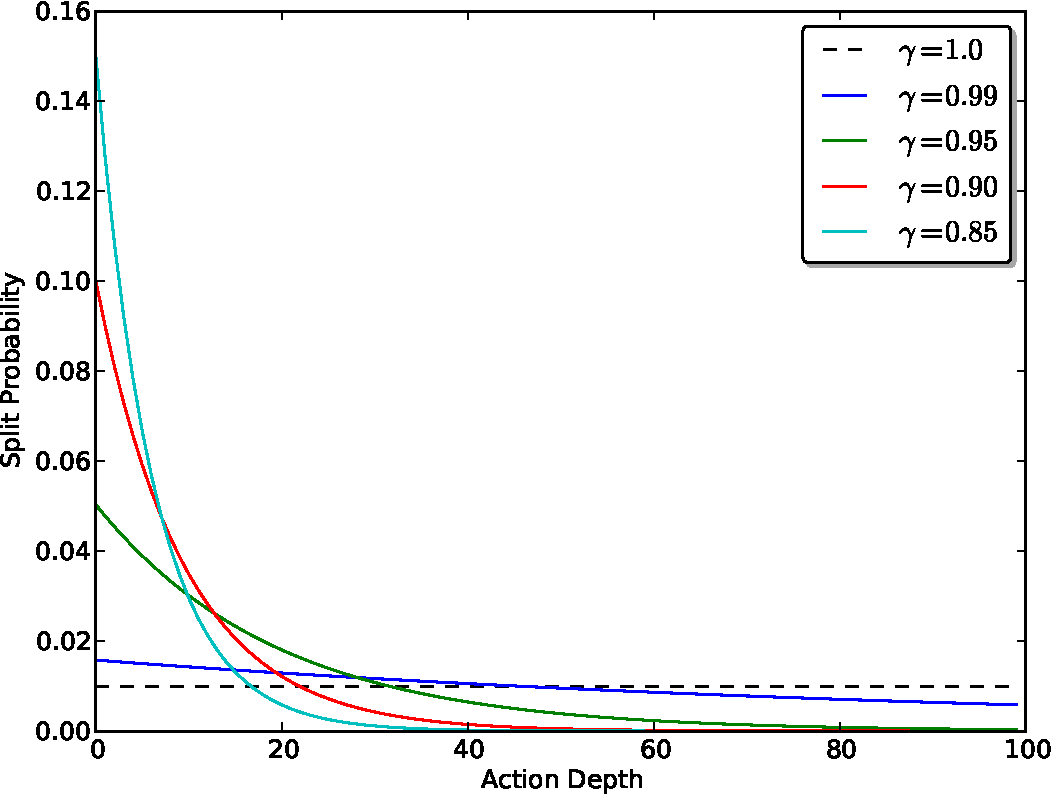
\includegraphics[width=0.45\textwidth]{graphics/gamma-crop.pdf}
  \caption{Examples of how rewards are affected by $\gamma$.}
  \label{fig:gamma}
\end{figure}


\subsection{Taxonomy of Planning Algorithms}
The terminology of Chang~\cite{chang2007simulation} is followed when trying to classify planning algorithms. If the policy $\pi:S \times A \rightarrow [0,1]$ is followed, what is known as ``closed loop'' planning takes place. The agent takes an action, senses its environment, takes another action etc. An alternative to closed-loop planning, ``open-loop'' planning, requires defining time. An agent sees a ``time'' when it's about to act instead of a state, i.e it doesn't have access to $s_t$, but just $t$. An open loop policy (or plan or control) is when an agent learns a policy with the form $\pi_o:S \times \mathcal{T} \rightarrow [0,1]$, where  $\mathcal{T}$ is an ordered set of time steps. Thus, an agent takes actions irrespective of the current state it is in. Intuitively this means that a sequence of actions is formed by the agent and the agent will take these actions in sequence (e.g. $(a_1,a_2,a_3,a_4,a_5,a_6,\dots,a_n)$). Obviously this is not optimal\footnote{Not optimal in the general case. It is optimal under the condition that the MDP is deterministic, i.e. each action leads to one specific state with probability one, and everything else has a probability zero}, although sometimes is much easier to do.


Another point of interest is planning, and when it happens. In open loop planning (and what is usually termed ``planning'' without any further qualifications), an agent forms a plan once and follows it until the end.

If the agent replans at every step, discarding or augmenting the plan received from previous steps, it is known as ``rolling horizon'' planning. The idea here is that, if the agent can plan as well as possible up to a  certain point, it can perform an action, move the planning horizon one step forward and replan. For example, Monte Carlo Tree Search for infinite MDPs can be seen as an approximate rolling horizon planning version of $TD(1)$\cite{silver2009reinforcement}.  The term ``Simulation based'' is used when the planning happens for an MDP that has a tree like structure and rewards are only visible at the end of the tree, a situation common in many games.

When learning how to act using a generative model, one can make a third distinction as to the type of sets represented by $A$ and $S$. In this paper the focus is on an $A$ and $S$ that come from a metric space. This means  that both sets' elements define a notion of distance and, for all practical purposes, have an infinite amount of elements. More specifically, both sets are drawn from a bounded set of real numbers, $\Re^n$.

Since an open loop policy is now a real-valued vector of actions, algorithms like T-HOO and CMA-ES can be used to find such a policy, hence the title of this paper. To the best of our knowledge this is the first time evolution has been used in such a setting. There are examples of closed loop rolling horizon papers, but these are beyond the scope of this article~\cite{xiang2012differential,samothrakis2010planning}.



\subsection{Notes on planning using a Generative Model}

The Markov Decision Process simply describes an environment alongside the rewards that said environment provides to an agent. A problem central to Artificial Intelligence is what actions an agent must take to maximise its long term reward. The most basic assumption one can make is that the agent knows nothing about the environment. In this case the agent gets thrown into the environment and interacts (``trains'') for some time. After the training is complete, the agent should be able to act intelligently (presumably with some success).

Another approach one can take is to assume that the agent has a copy of the MDP in its ``mind'' and thus is able to plan accordingly. This is usually termed dynamic programming~\cite{sutton1998reinforcement}, however it cannot be used in the case of continuous states or actions without the use of a function approximator (FA) or some kind of discretization. Another approach, and one which has made a significant impact recently, arguably presented for the first time by Kearns~\cite{citeulike:1584916} and popularised mostly as Upper Confidence Bounds for Trees (UCT)~\cite{kocsis2006bandit}, is to use a generative model.

A generative model is nothing more than a simulator of future events. This is a less of a requirement than knowing the full model (which entails knowing the full function $T$), but still requires the agent to have some knowledge of the world. This category of algorithms, which are broadly termed ``Rolling Horizon'', has the following steps. From the current state, a number of simulations of possible futures is run by executing a set of action sequences (all of this in the ``mind'' of the agent). The simulations last for a certain number of steps (hence the ``rolling horizon'') or continue until an end state is encountered (i.e. when the MDP has ``absorbing'' states that cannot be acted from).

Once a satisfactory plan/policy has been estimated (or the agent runs out of time, iterations etc. ) it proceeds by executing the first action of the plan, thus moving to the next state. Once there, the agent performs the same sequence of ``mental'' actions, (i.e. plans and executes the first action), until some predefined stopping condition.  In this paper we will concern ourselves \textit{only} with this method of planning. What changes from method to method is how the plan is formed. The main version of the algorithm used can be seen in Algorithm \ref{algo:ooop}.

In standard UCT, a procedure similar to temporal difference learning is followed (or, more closely, monte carlo methods), where one learns the value of each state. An agent then forms a policy by choosing a value greedily. In our case, because our state space has continuous states and actions, this is impossible without the use of a function approximator (or an infinite discretization of space), which is not attempted here. What is attempted though is to learn the policy function directly without reference to state, while planning continuously from the current state. So while the agent forms open-loop plans at each clock tick, in reality it is executing a closed-loop policy. While the strategy is not provably optimal, it can work well in practice~\cite{weinstein2012bandit}. This will be seen by our experimental results (see Section \ref{sec:Experiments}). 



\begin{algorithm}[!ht]
\caption{Rolling Horizon Open Loop Planning}\label{algo:ooop}
\begin{algorithmic}

\State 	\textbf{define external function} $\mathsc{FindOpenLoopPlan} (depth, T',S') $ \Comment{Try to find the optimal policy. You can use either evolution or T-HOO here}


	\Procedure{$\mathsc{OOP}$} {}
		\While{$!StoppingCondition$}
		    \State $a \gets \mathsc{FindOpenLoopPlan}(depth, T',S')[0]$ \Comment{Execute first action of the policy}
		    \State $s \sim T(s'|s,a)$ \Comment{Stop only at an absorbing state}
		\EndWhile
		\State
	\EndProcedure



\end{algorithmic}
\end{algorithm}


\section{Methodology} \label{sec:methodology}
Our methodology is simple, yet efficient. We test T-HOLOP and EVO-P in two simple benchmark problems (see below for more) and Lunar Lander, a classic arcade game. 


\subsection{Simple Planning Benchmarking Problems}

% % \todo[inline]{Simon to do this}.




For direct comparison with recent work on sample based planning using trees, in particular
Weinstein and Littman~\cite{weinstein2012bandit} and Pazis and Lagoudakis \cite{PazisBAS},
we used the same problems: double integrator, and inverted pendulum.  The basic
experimental setup followed Weinstein and Littman~\cite{weinstein2012bandit}
and Pazis and Lagoudakis \cite{PazisBAS}
closely, except that they used a fixed noise level for each experiment whereas we varied the
noise level to explore how performance was affected.

Both problems are modelled
using continuous state discrete time simulations.  In each case the desired
acceleration is corrupted by additive uniform random noise
before being limited within the specified range.  The noise levels are described in the next section.


\subsubsection{Double Integrator}

The double integrator problem is to control a mass along a single dimension.  The state space
is 2-dimensional, consisting of $(p,v)$ where $p$ is position and $v$ is velocity.
The goal is to change the state from $(1,0)$ to $(0,0)$.  Both position and velocity
are clamped to be within the range $-2$ to $+2$.  At each time step the controller selects
the desired acceleration $a'$, which then is noise corrupted and range limited between $-1.5N$ to $+1.5$N to yield the
applied acceleration $a$.

Euler integration is then used to update the position and velocity, given the time step $\delta_t$:

\begin{eqnarray}
v_{t+\delta_t} & = & v_{t} + a \delta_t \\
p_{t+\delta_t} & = & p_{t} + v_{t+\delta_t} \delta_t
\end{eqnarray}

At each time step the reward $r$ is:
\begin{equation}
 r = -(p^2 + a^2)
\end{equation}

The problem becomes harder as the time interval $\delta_t$ at %word missing?
each action is applied increases,
and following Pazis and Lagoudakis we set $(\delta_t = 0.5s)$.

% \begin{equation}
% R = -(p^2 + a^2)
% \end{equation}

\subsubsection{Inverted Pendulum}

The inverted pendulum problem is also known as the pole balancing
or cart-pole problem.  The goal is to keep the pendulum / pole as upright and as still as possible.
This is achieved by accelerating the cart which affects the freely pivoted pendulum.

In this instance of the problem the controller only sees a two dimensional
state space, consisting of the
angle $\theta$ that the inverted pendulum deviates from the vertical, and the angular velocity
of the pendulum $\dot{\theta}$.
The controller selects the desired angular force $F$,
which is then corrupted by additive uniform random noise and limited in the range $-50N$ to $+50$N
so as to yield the applied angular force $u$.  The angular acceleration $\ddot{\theta}$ is then calculated
as follows:

\begin{equation}
\ddot{\theta} = \frac{g sin(\theta) - \alpha m l (\dot{\theta})^2 sin(2 \theta) / 2 - \alpha cos(\theta) u}
                     {4l/3 - \alpha m l  cos^2(\theta)}
\end{equation}

where $g$ is the acceleration due to gravity
$(g = 9.8ms^{-2})$,
$m$ is the mass of the pendulum
$(m = 2kg)$, $(\alpha = 1 / (m + M))$, $M$ is the mass of the cart
$(M = 8kg)$ and $l$ is the length of the pendulum $(l = 0.5m)$.
The time interval $\delta_t$ was set to $0.1s$: i.e.\ the simulation is
updated 10 times per second:

\begin{eqnarray}
\dot{\theta}_{t+\delta_t} & = &  \dot{\theta}_{t} + \ddot{\theta} \delta_t \\
\theta_{t+\delta_t}  & = & \theta_{t} + \dot{\theta}_{t+\delta_t} \delta_t
\end{eqnarray}

At each timestep the reward $r$ punishes deviation from the vertical, high speed, and high force:
\begin{equation}
r = -((2 \theta / \pi)^2 + \dot{\theta}^2 + (F / 50)^2 )
\label{eq:rew:t}
\end{equation}


\subsection{Lunar Lander}
We describe the properties of Lunar Lander. 

\subsubsection{Environmental Properties}

The properties of the base environment of {\itshape Lunar Lander} are that it is frictionless, and that it is a two-dimensional plane with horizontal wrapping. This can also be conceptualised as a cylinder. Anything that passes from the left edge of the playing field moves to the right instantaneously, and vice versa.

The other feature of note is the jagged landscape, a simplistic representation of the noisy, crater-filled lunar landscape the game represents. This landscape is constructed as a series of line segments, with each vertex of the jagged landscape being distributed equally horizontally, and randomly vertically. % unclear?

% TODO: DIAGRAM - jagged lunar landscape might be useful (reuse of old one probably not sufficient)

% not sure how much detail should be gone into here? should just cite generation equations from old paper or copy over??

Each vertex of this landscape is generated sequentially. % INCOMPLETE due to uncertainty listed above


\subsubsection{Spaceship Physics}

The spaceship within this game world is modelled as an a circular mass with some basic physical properties, such as a position within the game world $\boldsymbol {s}$, a velocity $\boldsymbol {v}$, an orientation $\theta$, an angular velocity $\omega$ and a radius of a bounding sphere $r$ used for collision detection with the landscape.

This collision detection method is based on the lowest point of the spaceship's bounding circle coming into intersection with the highest point of the landscape for the line perpendicular between the ship and the bottom of the playing field, as can be seen in Figure \ref{fig:diagram_landscapepoint}.

% this needs a diagram for clarity: reuse the old one? reusing it temporarily
\begin{figure}[hbtp]
\centering
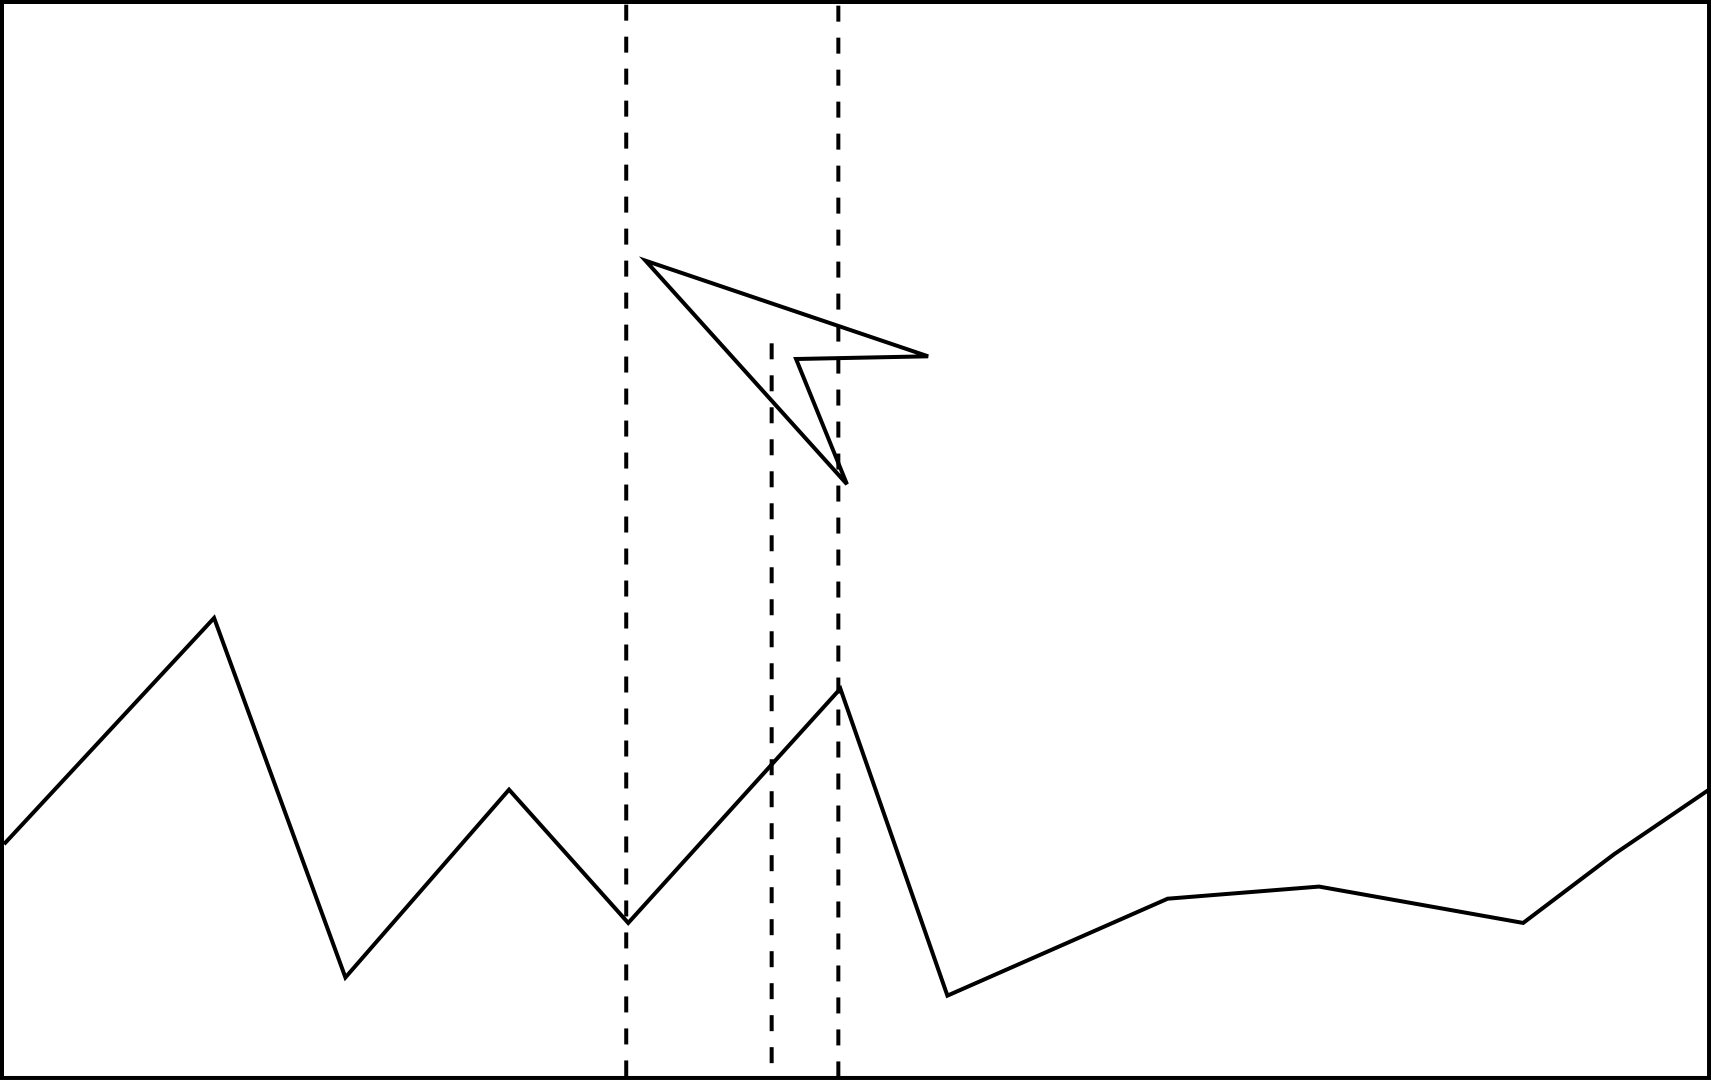
\includegraphics[scale=0.4]{graphics/landscapepoint}
\caption{The point closest to the spaceship on the landscape lies in between two of the defined vertices of the landscape, and requires interpolation to calculate the y co-ordinate from the x co-ordinate of the ship.}
\label{fig:diagram_landscapepoint}
\end{figure}

As the landscape is stored as a series of line segments, interpolation must be used in the event the ship is not perfectly aligned with one of the landscape axes. The point that lies on the line segment that the ship is being checked against is calculated through simple linear interpolation based on which two vertices the ship is horizontally closest to. For the ship's centre $\boldsymbol {s}$, the left nearest landscape vertex $\boldsymbol {p}^{l}$ and the right nearest landscape vertex $\boldsymbol {p}^{r}$, the point of collision $\boldsymbol {p}^{c}$ against the landscape is calculated as 

% does this constitute self-plaigarism???


\begin{figure*}[ht]
  %\centering



  \centering
        \begin{subfigure}[b]{0.32\textwidth}
                \centering
                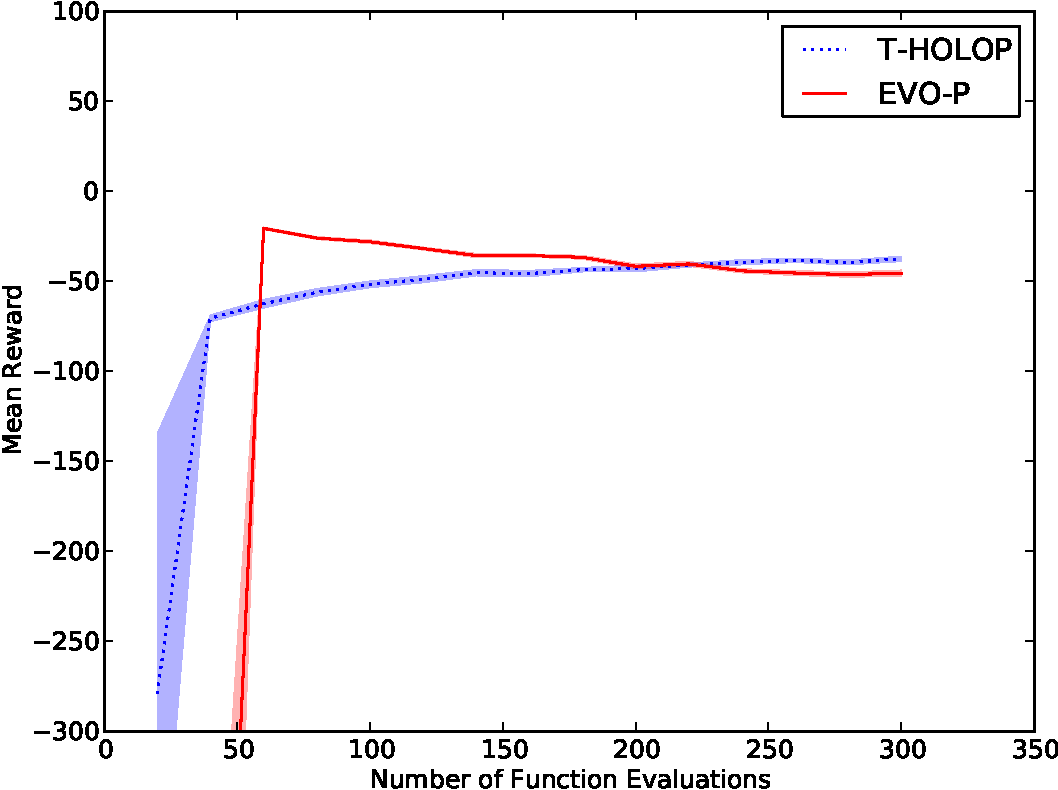
\includegraphics[width=1.0\textwidth]{graphics/online-IP-crop.pdf}
                \caption{Scores for a noise level of $l=1$ under variable function evaluations. }
                \label{fig:IP}
        \end{subfigure}   \begin{subfigure}[b]{0.32\textwidth}
                \centering
                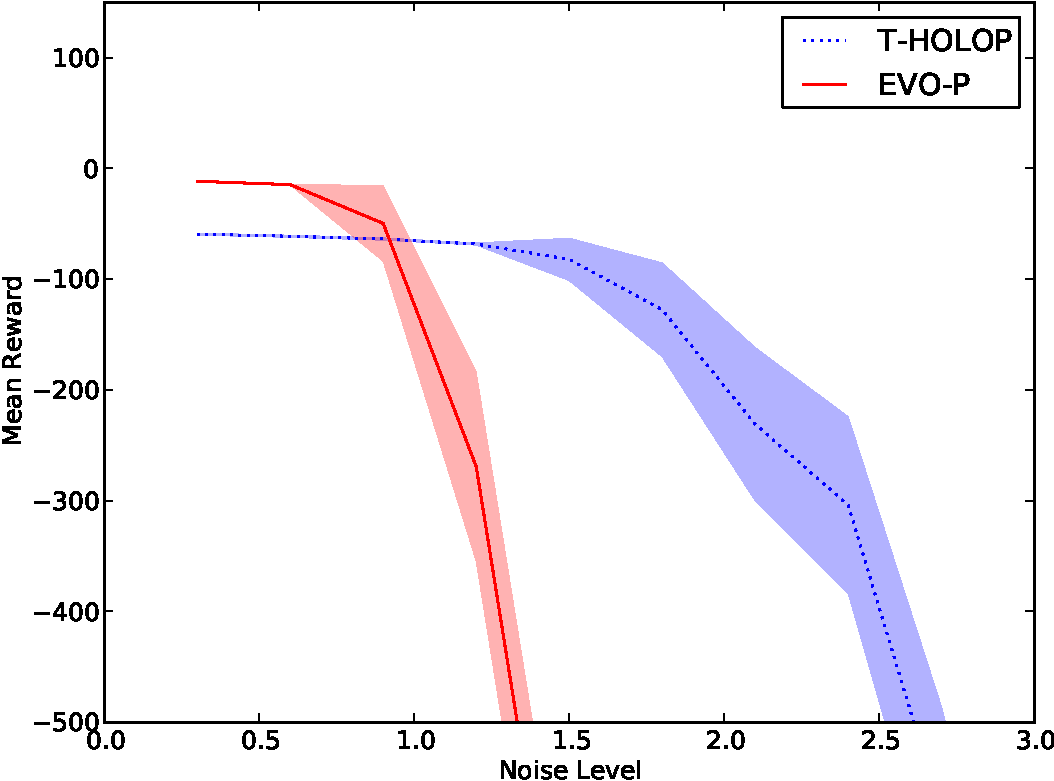
\includegraphics[width=1.0\textwidth]{graphics/online-noise-IP_50-crop.pdf}
                \caption{Scores for 50 iterations under variable noise level $l$.}
                \label{fig:IP-N-50}
        \end{subfigure}  \begin{subfigure}[b]{0.32\textwidth}
                \centering
                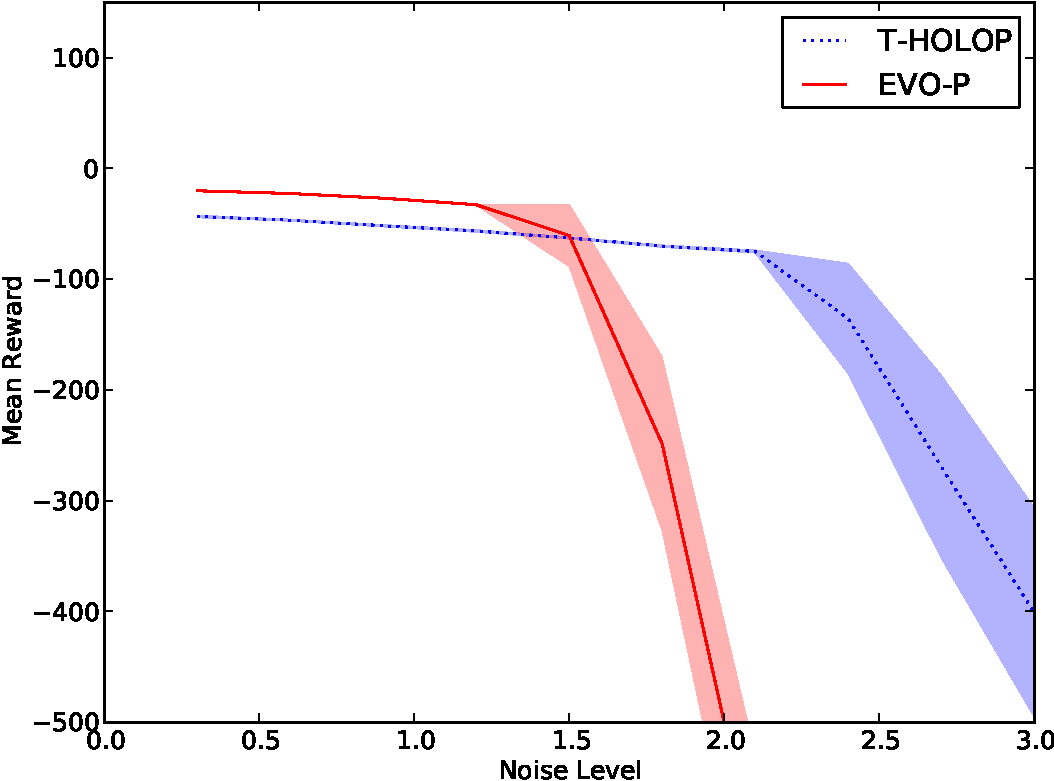
\includegraphics[width=1.0\textwidth]{graphics/online-noise-IP_100-crop.pdf}
                \caption{Score for 100 iterations under variable noise level $l$.}
                \label{fig:IP-N-100}
        \end{subfigure}%

         \caption{Performance of both T-HOLOP and EVO-P in the Inverted Pendulum benchmark (error bars for the 95th percentile). Higher scores are better}
         \label{fig:IP-all}

\end{figure*}


        \begin{figure*}[ht]

        \begin{subfigure}[b]{0.32\textwidth}
                \centering
                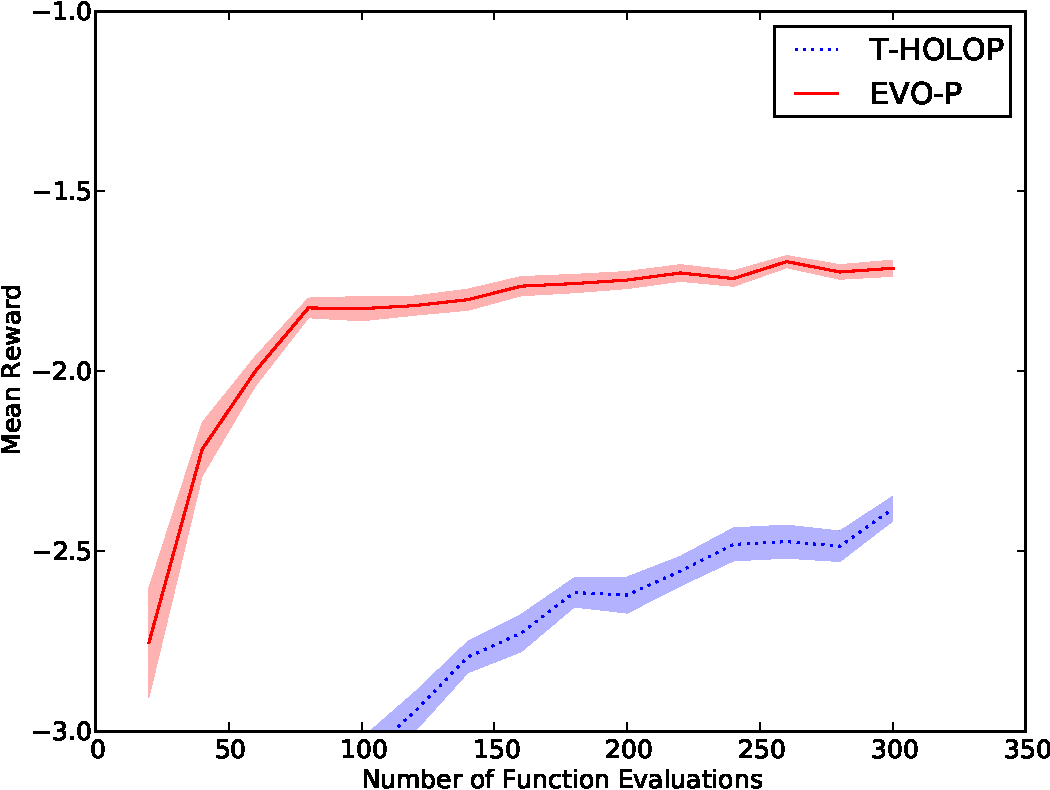
\includegraphics[width=1.0\textwidth]{graphics/online-DI-crop.pdf}
                \caption{Scores for a noise level of 1 under variable function evaluations.}
                \label{fig:DI}
        \end{subfigure}   \begin{subfigure}[b]{0.32\textwidth}
                \centering
                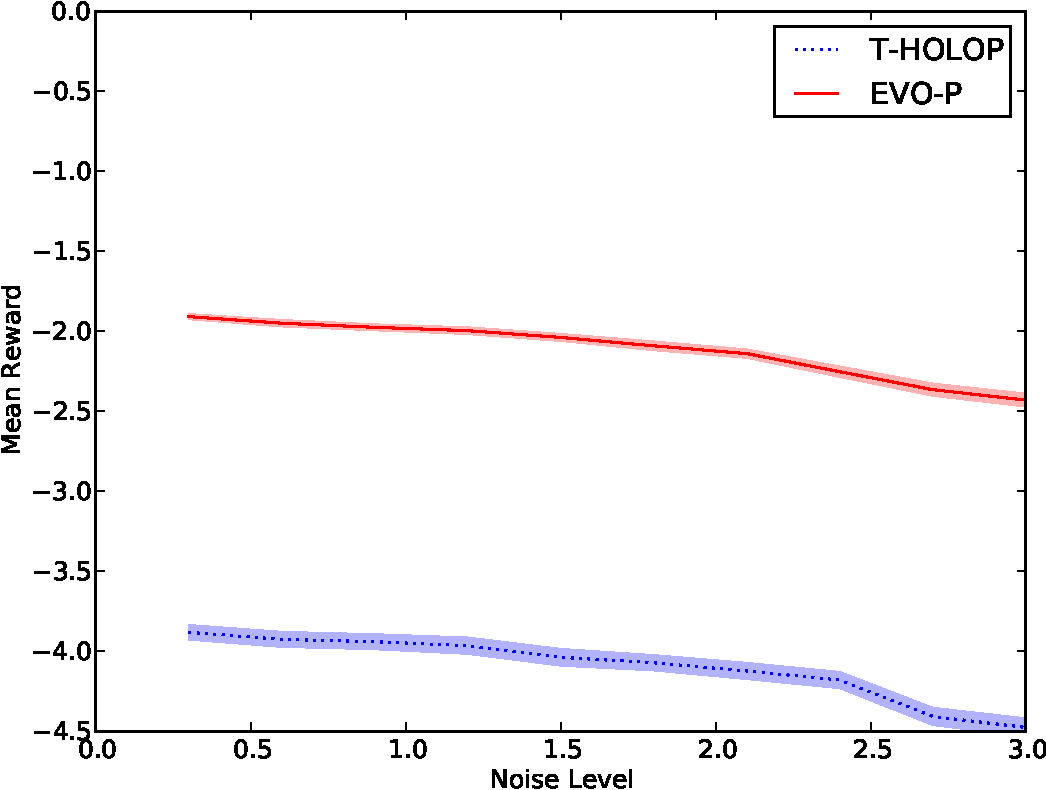
\includegraphics[width=1.0\textwidth]{graphics/online-noise-DI_50-crop.pdf}
                  \caption{Scores for 50 iterations under variable noise level $l$. }
                \label{fig:DI-N-50}
        \end{subfigure}   \begin{subfigure}[b]{0.32\textwidth}
                \centering
                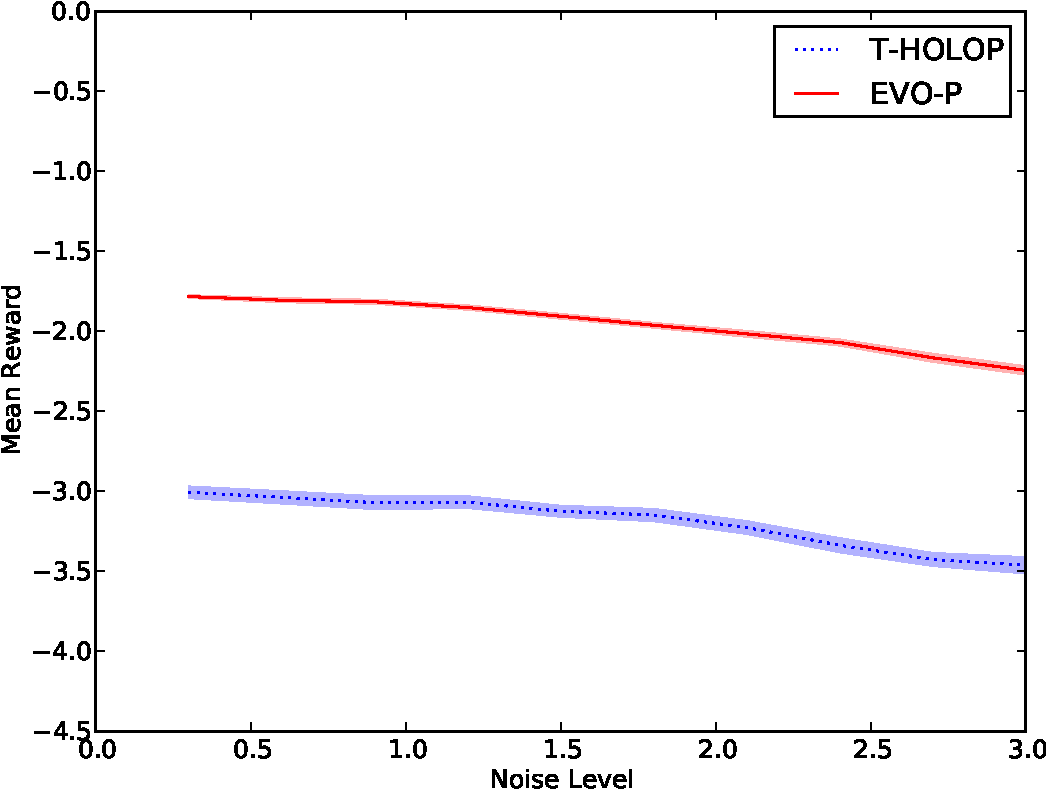
\includegraphics[width=1.0\textwidth]{graphics/online-noise-DI_100-crop.pdf}
                \caption{Score for 100 iterations an variable noise level $l$.}
                \label{fig:DI-N-100}
        \end{subfigure}

  \label{fig:DI-all}

       \caption{Performance of all algorithms in the Double Integrator benchmark (error bars for the 95th percentile). Higher scores are better}


\end{figure*}

\begin{equation}
\boldsymbol {p}_{x}^{c} = \boldsymbol {s}_{x}
\boldsymbol {p}_{y}^{c} = \boldsymbol {p}_{y}^{l} + v(\boldsymbol {p}_{y}^{r} - \boldsymbol {p}_{y}^{l})
\end{equation}

where $v$ is a value between $0$ to $1$ used for interpolation, and can be calculated as follows.

\begin{equation}
v = \frac{ {\boldsymbol {s}_{x} - \boldsymbol {p}_{x}^{l}}}{ {\boldsymbol {p}_{x}^{r} - \boldsymbol {p}_{x}^{l}} }
\end{equation}

Collision is then true if the following statement is true:

\begin{equation}
\boldsymbol {s}_{y} + r \geq \boldsymbol {p}^{c}_{y}
\end{equation}

The ship colliding with the landscape constitutes the end of the {\itshape Lunar Lander} game. The conditions surrounding this collision, including speed, orientation of the ship, and fuel used, constitute whether the nature of the collision is a success or a failure.

An agent can modify the ship directions by applying linear thrust $\bm{a_T}$ and the angular impulse $\bm{a_I}$. The controllers have to identify a vector of real numbers $\bm{A}$, which each element of the set $a_i \in [0,1]$. Each even element of the vector represents the linear thrust, whereas each odd element represents angular velocity. Each linear thrust vector element is transformed by applying as follows: 

\begin{equation}
\bm{a_I} = 5(\bm{a_I} - 0.5)
\bm{a_T} = 300\bm{a_T} 
\end{equation}

Finally each linear thrust and angular impulse is repeated for $X$ actions, the effects of which we are going to explore below. 

\subsubsection{Heuristic} % this too

Lunar Lander has a setup where a player gets rewards if and only if it actually lands on the pad. This creates the problem of rollouts (whether used by EVO-P or T-HOLOP) rarely will see a reward. In order to circumvent this, as it is common in other games, we use a heuristic for each state. In order to counter this tendency, as is common in games, we used a two-stage heuristic. The first stage involves the ship trying to reach the landing pad. 


\begin{multline}
rng = -\sum{arccos(vl\cdot\theta)/||vl||*||\theta||} - |\boldsymbol {v_y} - V_{y}^{max}| \\
h = \twopartdef{ -|(|\boldsymbol {v}| - C) - |\boldsymbol {s}_{x} - \boldsymbol {np}_{x}||}{||\boldsymbol {s} - \boldsymbol {np}|| < D}
{rng - |\boldsymbol {v_x}|   }{Otherwise}
\label{eq:h1}
\end{multline}

In the above Equation \ref{eq:h1} the constant C denotes the maximum magnitute of speed, which we set to $C=100$. $D = 60$ is the distance from the landing point $np$ where this heuristic takes precedence.  Intuitively, the upper part of the heuristic $h$ tries to get the ship above the landing point as fast as possible while maintaining a certain speed. The second part of the heuristic tries to minimise velocity on the $x$ axis (as the ship tries to land), maintain a minimum landing speed on the $y$ axis and get a certain angle (the summation term $rng$) as close to vector $vl = (0,-1)$, i.e. help the ship stay upright through the duration of the rollout.  

\section{Results} \label{sec:Experiments}
We present the results of our experiments below.

\begin{table}
	\begin{tabular}{lrrrr}
\hline
 Map Name   &   Success Mean &   Success CI &   Ticks Mean &   Tick CI \\
\hline
 map2       &            1   &     0        &       2925.9 &   184.437 \\
 map1-tall  &            1   &     0        &       2733   &   159.34  \\
 map1-easy  &            1   &     0        &       2293   &   123.917 \\
 map1-wall  &            0.9 &     0.226216 &       2421.6 &   682.893 \\
\hline
\end{tabular}
\end{table}



% \begin{figure*}[ht]
%   %\centering



%   \centering
%         \begin{subfigure}{0.49\textwidth}
%                 \centering
%                 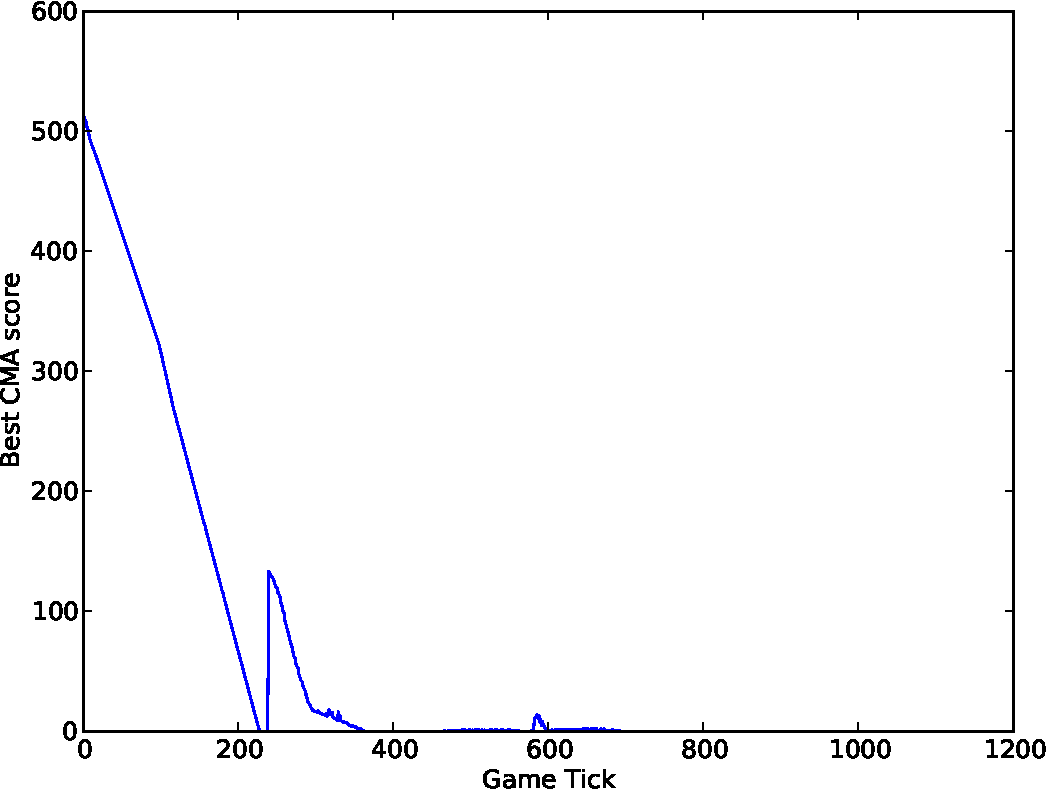
\includegraphics[width=1.0\textwidth]{./lunarexps/sample-crop.pdf}
%                 \caption{Best value for each tick EVO-P could find. }
%                 \label{fig:sample}
%         \end{subfigure}  
%         \begin{subfigure}{0.49\textwidth}
%                 \centering
%                 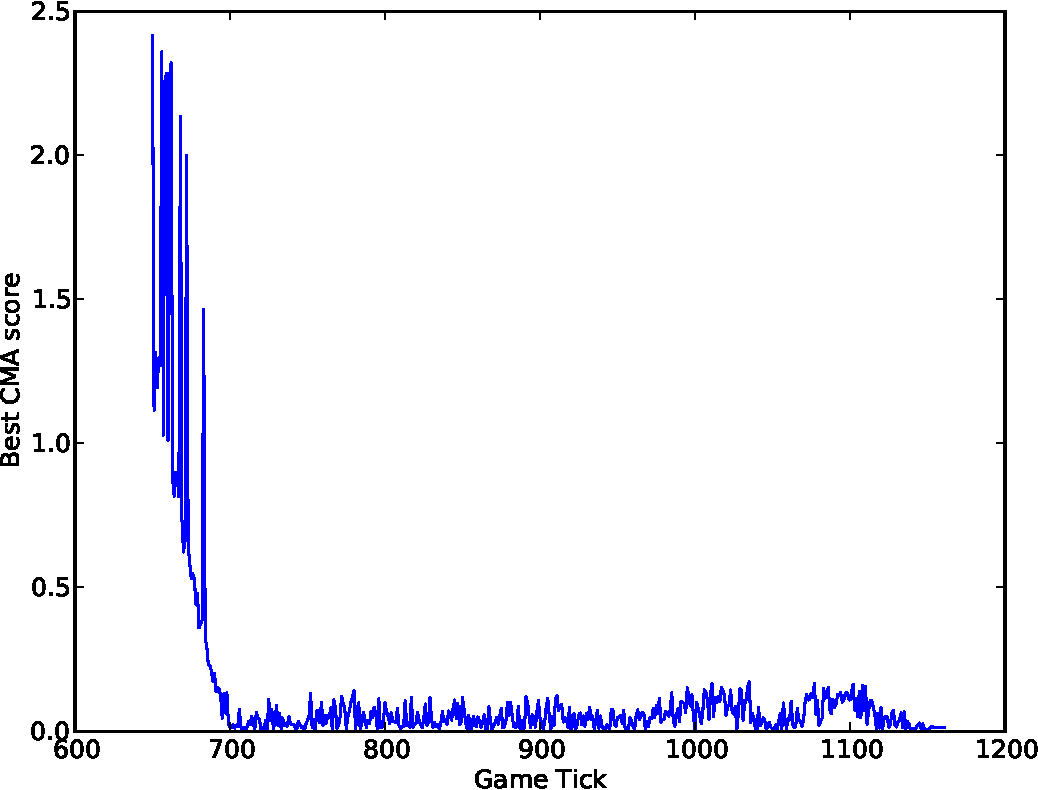
\includegraphics[width=1.0\textwidth]{./lunarexps/sample-detail-crop.pdf}
%                 \caption{Detail of Figure \ref{fig:sample}, when the ship is closer to landing.}
%                 \label{fig:sample-detail}

%         \end{subfigure}
       

%          \caption{Sample run for EVO-P. Best fitness discovered at each tick is shown. Notice the big ``bump'' in fitness when the ship gets close to the landing pad}
%          \label{fig:samples}

% \end{figure*}


\begin{figure*}[ht]
  \centering



  \centering
        \begin{subfigure}{0.49\textwidth}
                \centering
                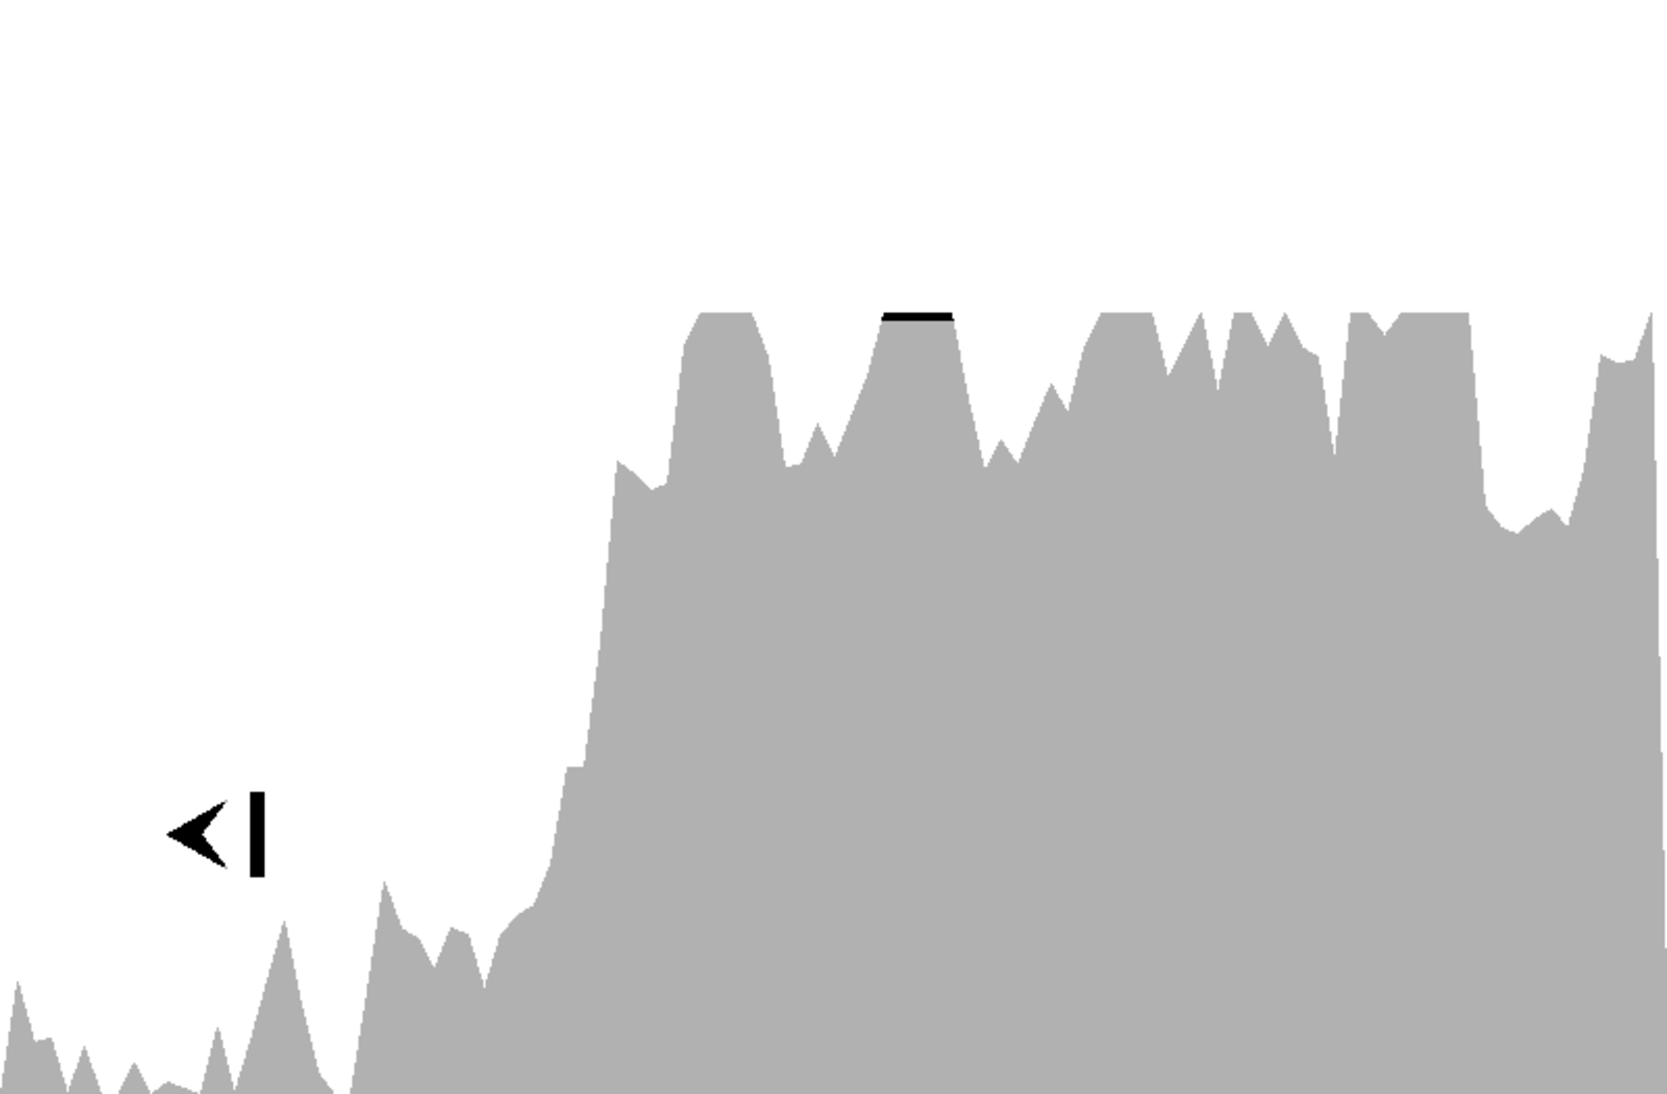
\includegraphics[width=1.0\textwidth]{./graphics/map2.pdf}
                \caption{Map. }
                \label{fig:map2}
        \end{subfigure}  
        \begin{subfigure}{0.49\textwidth}
                \centering
                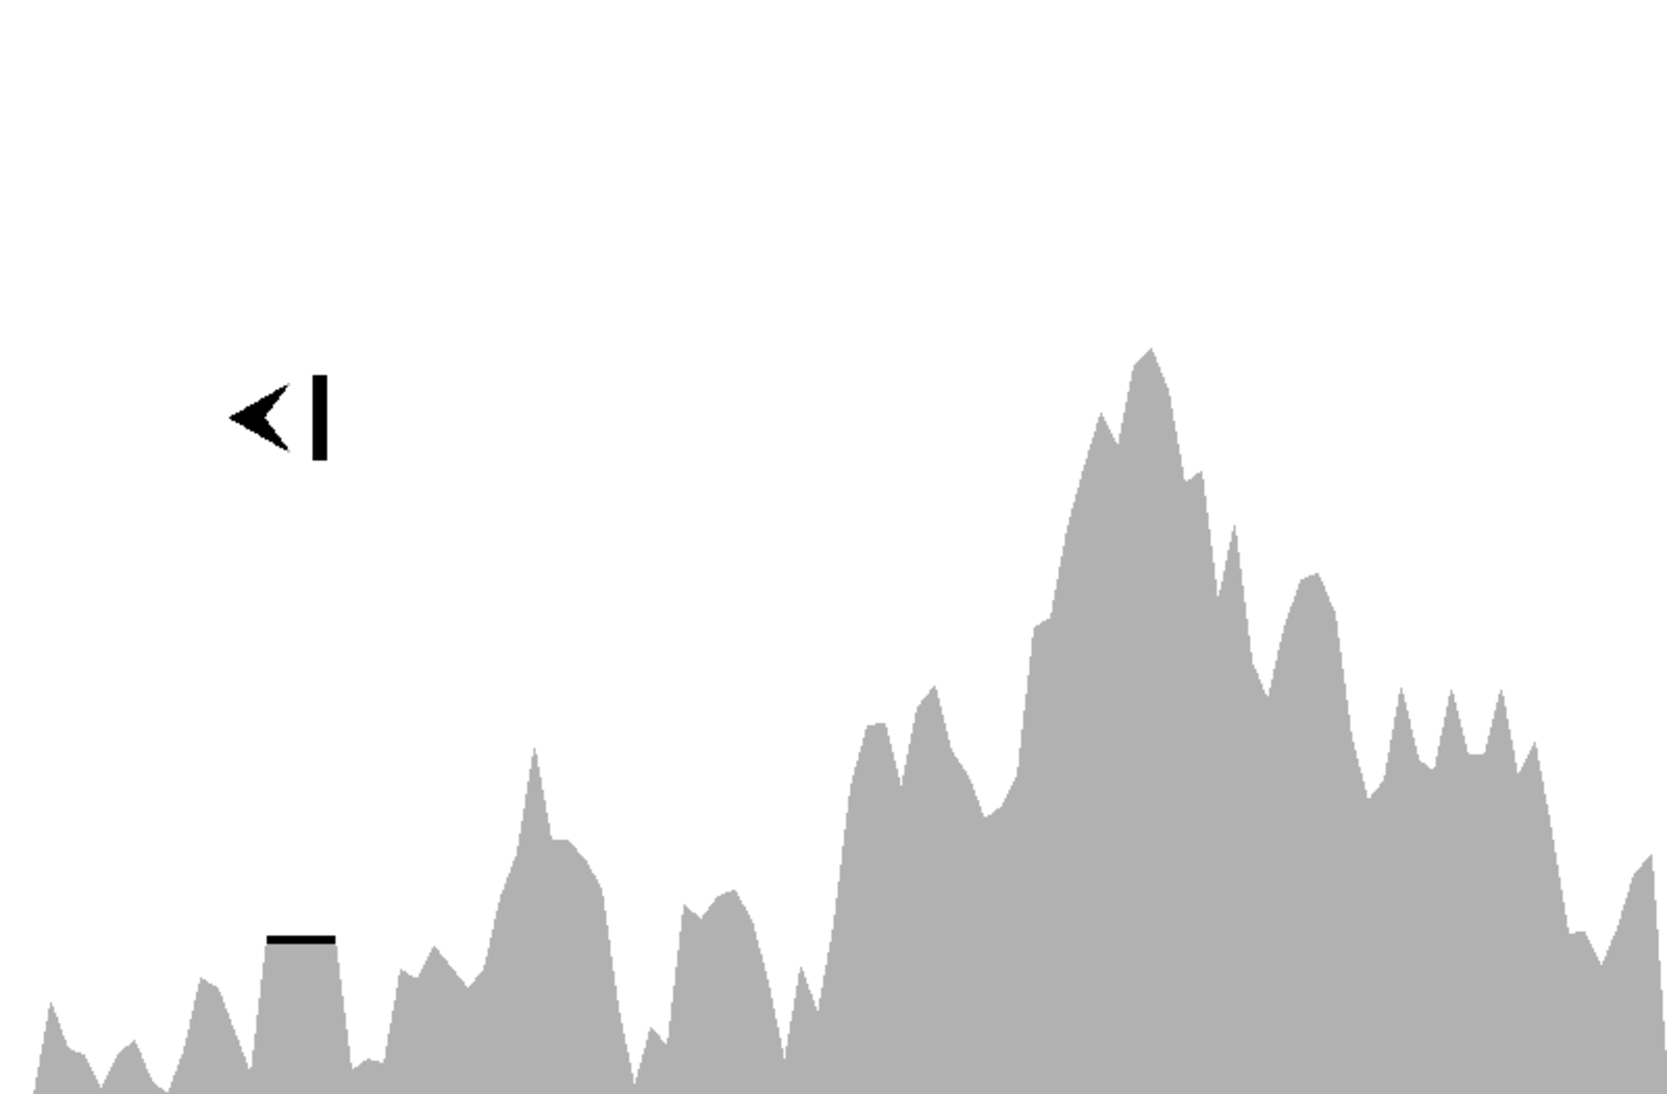
\includegraphics[width=1.0\textwidth]{./graphics/map1-easy.pdf}
                \caption{sdfdf}
                \label{fig:map1-easy}

        \end{subfigure}
\\
        \begin{subfigure}{0.49\textwidth}
                \centering
                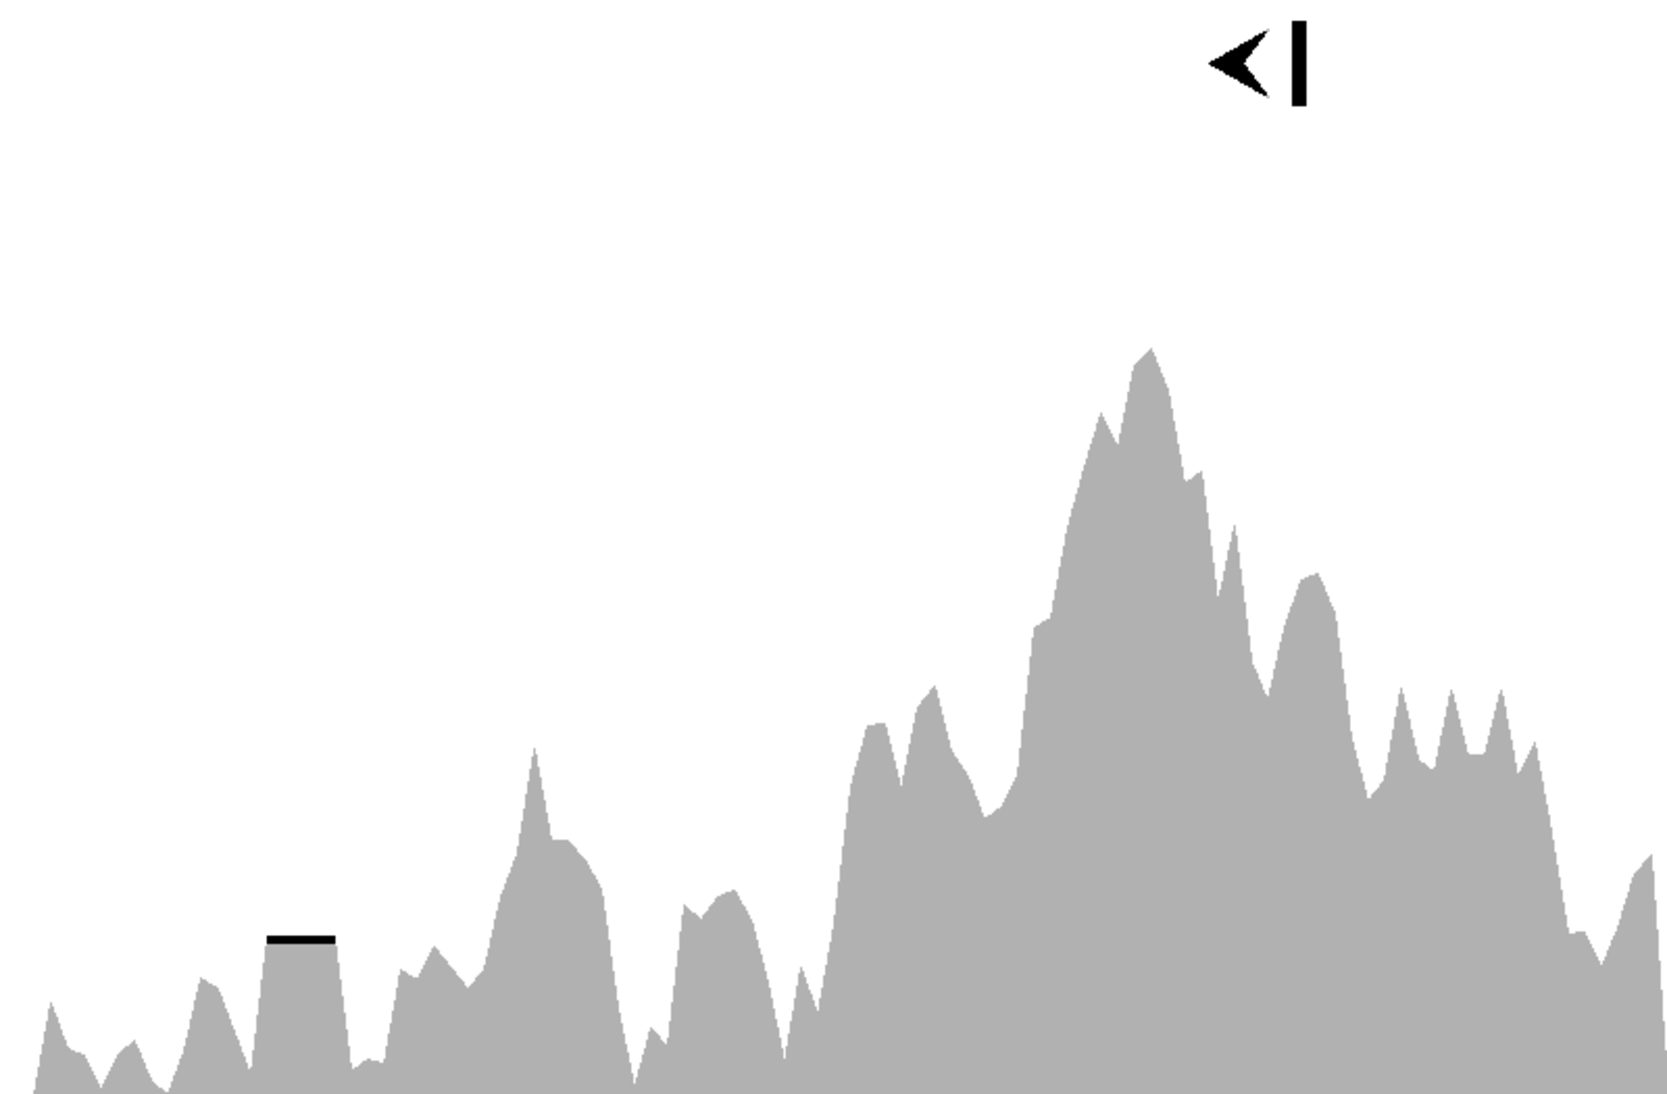
\includegraphics[width=1.0\textwidth]{./graphics/map1-tall.pdf}
                \caption{Detail of Figure \ref{fig:sample}, when the ship is closer to landing.}
                \label{fig:map1-tall}\end{subfigure}\begin{subfigure}{0.49\textwidth}
                \centering
                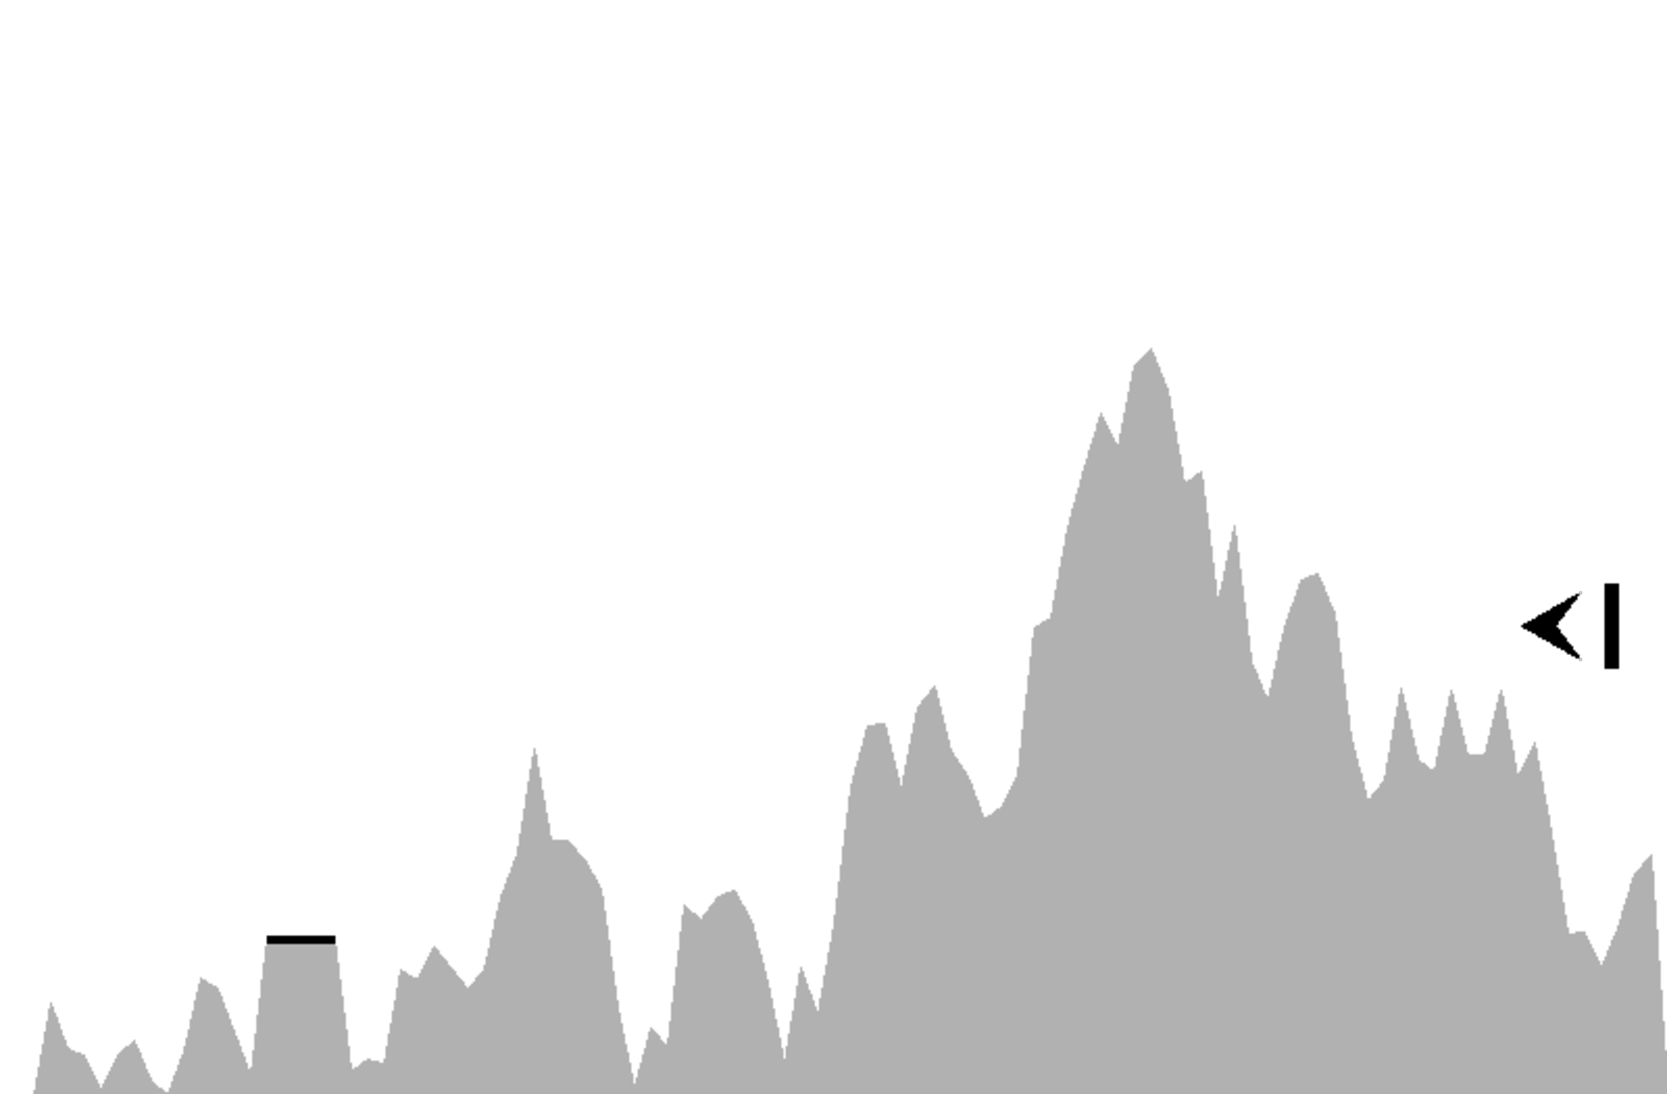
\includegraphics[width=1.0\textwidth]{./graphics/map1-wall.pdf}
                \caption{Detail of Figure \ref{fig:sample}, when the ship is closer to landing.}
                \label{fig:map-wall}

        \end{subfigure}
       

         \caption{Sample run for EVO-P. Best fitness discovered at each tick is shown. Notice the big ``bump'' in fitness when the ship gets close to the landing pad}
         \label{fig:maps}

\end{figure*}

\subsection{Benchmark Problems}


For the second set of experiments we have defined the following variables. The first two involve running the experiments with a fixed rollout depth of 50, i.e. each algorithm at each step plans for 50 steps ahead. We set the noise levels to $0.1 (\mathcal{U}(0,1)-0.5)*2 l$ uniform noise for the double integrator experiment and $10 (\mathcal{U}(0,1)-0.5)*2 l$  for the Inverted Pendulum.  The variable $l$ is the noise level which defines how noisy the environment is. Initially, we performed two experiments, with a variable number of iterations and a fixed noise level of one. 

An example of how the \textit{predicted} reward looks like for a $2$-step look-ahead (instead of $50$ we use in the experiments) can be seen in Figure \ref{fig:vis}. We plotted the full state-space by pushing the internal generative model two steps forward for all possible actions by discretizing each action. Notice how the predicted reward landscape changes over time as the agent moves. The continuous replanning should aim to perform the action with the highest future reward.  



The results of these experiments can be seen in graphs  \ref{fig:IP} and \ref{fig:DI}. These are close to the original experiments of Weinstein and Littman~\cite{weinstein2012bandit}, only this time we varied the number
of iterations allowed for each algorithm. The original experiment had given the algorithms 200 value iterations. With this number of iterations, for the Inverted Pendulum experiment the mean reported (using HOLOP) was $-47.45$. We got a better mean using T-HOLOP
% % \footnote{We believe there is a minor bug in the HOLOP implementation Weinstein et al use.}
\footnote{This was due to a minor difference between our implementation of HOLOP and Weinstein's.}
 of $-42.94$.

 EVO-P got as score of $-41.69$. It also  seems to have a drop in performance as we increase function evaluations, presumably because it converges to a false minima without any uncertainty handling mechanism to stop this. This kind of behaviour has been observed previously in Evolutionary Algorithms~\cite{hansen2009tec} when having noisy function.

For the double integrator experiment, we had slightly different results. The Weinstein paper reports a mean of $-2.72$ for 200 iterations. Using T-HOLOP we got a better mean of $-2.62$. A far better result of $-1.74$ is obtained by EVO-P. 


Results for the variable noise levels $l$ (Figures \ref{fig:IP-N-50}, \ref{fig:IP-N-100}, \ref{fig:DI-N-50}, \ref{fig:DI-N-100}) closely mimic the performance of their constant noise counterparts. For the inverted pendulum, using just 50 iterations (Figure \ref{fig:IP-N-50}) EVO-P is able to stabilise the pendulum with . This still applies if we increase the number of function evaluations to 100 (Figure \ref{fig:DI-N-100}). On the other hand, the results start to get closer to the fixed noise level experiments if we increase the number of iterations in the Inverted Pendulum experiment to 100 (Figure \ref{fig:IP-N-50}).




\section{Conclusion} \label{sec:conclusion}

 
% Use \section* for the acknowledgments
\section*{Acknowledgements}
This work was supported by EPSRC grant EP/H048588/1 entitled:``UCT for Games and Beyond'' and an EPSRC Ph.D studentship. 



\bibliographystyle{IEEEtran}
\bibliography{lunarcontbib}
\end{document}